% Created 2017-09-11 Mon 14:46
\documentclass[9pt,lineo]{elife}

\usepackage{amsmath}
\usepackage{amssymb}
\usepackage[version=4]{mhchem}
\usepackage{siunitx}


              \usepackage[utf8]{inputenc}
\sisetup{detect-all}
\setcounter{secnumdepth}{0}
\date{\today}
\title{}
\hypersetup{
 pdfauthor={},
 pdftitle={},
 pdfkeywords={},
 pdfsubject={},
 pdfcreator={Emacs 25.1.2 (Org mode 8.3.5)}, 
 pdflang={English}}
\begin{document}

\begin{figure}
  \begin{fullwidth} \centering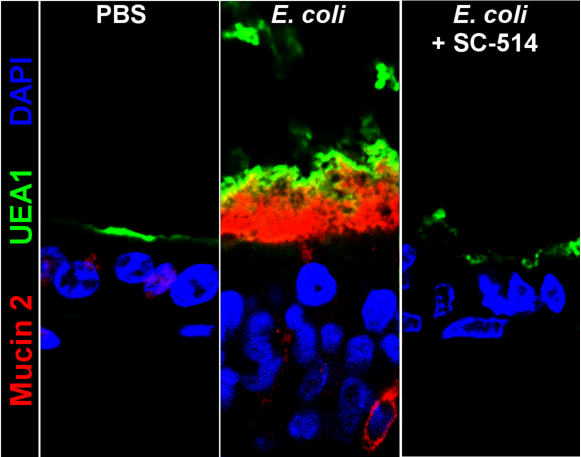
\includegraphics[width=0.9\linewidth]{./figures/figure7/Supplemental_Figure4_Muc2-NFkB.pdf}
\caption*{\textbf{Figure 7 - Supplement 1. }Representative confocal micrographs of HIOs treated as indicated. Fluorescent immunostaining pseudocoloring applied as indicated in the figure legend. 40X optical magnification with 3X digital zoom.}
\label{fig:fullwidth}
\end{fullwidth}
\end{figure}
\end{document}